\documentclass[report, notitlepage]{jlreq}
\usepackage{docmute}
\usepackage{global}
\usepackage{./sub/local}
\def\assetspath{./}
%\makeindex
%\makeglossaries

\title{常微分方程式}
\author{Yahata}
\date{2021S}

\begin{document}

\maketitle
\begin{abstract}
    常微分方程式についてまとめる。
\end{abstract}

\setcounter{tocdepth}{1}
\tableofcontents
\markboth{\contentsname}{}

% ============================================================
%
% ============================================================
\newpage
\documentclass[report]{jlreq}
\usepackage{../../global}
\usepackage{./local}
\subfiletrue
\def\assetspath{../}
%\makeindex
\begin{document}


\chapter{常微分方程式の基礎}

\section{常微分方程式とその解}

\begin{definition}[1.1.1 $n$階常微分方程式]
    関係式
    \begin{equation}
        f(x, y, y', \dots, y^{(n)}) = 0
    \end{equation}
    を\textbf{$n$階常微分方程式}という。
\end{definition}

\begin{problem}[例1.1.3]
    ヨウ素131の半減期は約8日である。10年後の時点で残っている割合を求めよ。

    解答:
    \begin{equation}
        \text{約}\, 2^{-365 \times 10 / 8} = 10^{-(3650 / 8) \times \log_{10} 2} < 10^{-100}
    \end{equation}
\end{problem}

\begin{problem}[例1.1.7]
    2階常微分方程式$my'' = -ky$を連立1階常微分方程式に書き直し、その解を求めよ。

    解答:
    \begin{equation}
        \begin{bmatrix}
            y_1 \\ y_2
        \end{bmatrix}
        =
        C_1 \begin{bmatrix}
            \sin \omega x \\
            \omega \cos \omega x
        \end{bmatrix}
        + C_2 \begin{bmatrix}
            \cos \omega x \\
            - \omega \sin \omega x
        \end{bmatrix}
        \quad \left(\omega = \sqrt{k / m}\right)
    \end{equation}
\end{problem}

\section{解の存在と一意性など}

\begin{definition}[1.2.1 正規形]
    \,
    \begin{enumerate}
        \item $n$階常微分方程式が\textbf{正規形}であるとは
            \begin{equation}
                y^{(n)} = f(x, y, \dots, y^{(n-1)})
            \end{equation}
            という形をしていること。
        \item $n$個の未知関数を持つ連立1階常微分方程式が\textbf{正規形}であるとは
            \begin{equation}
                y_j' = f_j(x, y_1, \dots, y_n)
            \end{equation}
            という形をしていること。
    \end{enumerate}
\end{definition}

この講義で扱う微分方程式は全て正規形に直せる。
以下、$\bm{x} = {}^t (x_1, \dots, x_n) \in \R^n$に対し
\begin{equation}
    \| \bm{x} \| \coloneqq \sum_{i=1}^n |x_i|
\end{equation}
とおく。

\begin{definition}[1.2.3 リプシッツ条件]
    $\alpha \in \R,\, \bm{\beta} \in \R^n$と
    $a \in \R_{>0},\, b \in \overline{\R}_{>0}$をとり
    \begin{equation}
        D \coloneqq \left\{
            \begin{pmatrix}
                x \\
                \bm{y}
            \end{pmatrix} \in \R^{n+1}
            \,\middle|\,
            |x-\alpha| \le a,\, \|\bm{y} - \bm{\beta}\| \le b
        \right\}
    \end{equation}
    とおく。
    $\bm{f}$が$D$上で\textbf{リプシッツ条件}をみたすとは、
    $\exists L > 0$\quad s.t.
    \begin{equation}
        \forall
            \begin{pmatrix}
                x \\
                \bm{y}
            \end{pmatrix},
        \forall
            \begin{pmatrix}
                x \\
                \bm{z}
            \end{pmatrix}
            \in D
        \quad \text{に対し} \quad
        \| \bm{f}(x, \bm{y}) - \bm{f}(x, \bm{z}) \| \le L \| \bm{y} - \bm{z} \|
    \end{equation}
    が成立することである。
\end{definition}

\begin{theorem}[1.2.5 解の存在と一意性]
    $\bf$を$D$上の連続関数とし、$D$上でリプシッツ条件をみたすとすると、
    初期値問題
    \begin{equation}
        \by' = \bf(x, \by),\quad \by(\alpha) = \bm{\beta}
        \label{1:eq:1}
    \end{equation}
    の解が、$[\alpha - \delta, \alpha + \delta]$上でただ1つ存在する。
    ただし、
    \begin{enumerate}
        \item $b = \infty$のとき$\delta = a$
        \item $b < \infty$のとき$\delta = \min\{a, b/M\},\, M = \max_{D} \| \bf(x, \bm{y}) \|$
    \end{enumerate}
    である。
\end{theorem}

定理の後半からわかるように、リプシッツ条件の成立範囲$D$と解の存在範囲は一般に一致しない。

\begin{proof}
    まず解の一意性を示そう。
    $\by,\, \wideby \colon [\alpha - \delta, \alpha + \delta] \to \R^n$を
    ふたつの解とすると、それらが式(\ref{1:eq:1})をみたすことから
    \begin{equation}
        \begin{split}
            \by(x) &= \beta + \int_\alpha^x \bf(t, \bm{y}(t))\, dt \\
            \wideby(x) &= \beta + \int_\alpha^x \bf(t, \wideby(t))\, dt
        \end{split}
    \end{equation}
    が成り立つ。これらの差を$\bm{z}(x) \coloneqq \by(x) - \wideby(x)$とおくと
    \begin{align}
        \|\bm{z}(x)\|
            &= \left\| \int_\alpha^x \left( \bf(t, \by(t)) - \bf(t, \wideby(t)) \right)\, dt \right\| \\
            &= \sum_i
                \left| \int_\alpha^x \left( f_i(t, \by(t)) - f_i(t, \wideby(t)) \right)\, dt \right| \\
            &\le \sum_i
                \left| \int_\alpha^x \left| f_i(t, \by(t)) - f_i(t, \wideby(t)) \right|\, dt \right| \\
            \intertext{外側の絶対値は$x \ge \alpha$ならば不要、$x < \alpha$ならばすべて負となるので}
            &= \left| \int_\alpha^x \left\| \bf(t, \by(t)) - \bf(t, \wideby(t)) \right\|\, dt \right| \\
            &\le L \left| \int_\alpha^x \| \bm{z}(t) \|\, dt \right|
                \label{1:eq:2}
    \end{align}
    となる。ただし、$L$はリプシッツ定数である。
    ここで$N \coloneqq \max_{|x - \alpha| \le \delta} \|\bm{z}(x)\|$とおくと、
    不等式(\ref{1:eq:2})を繰り返し用いることで
    \begin{equation}
        \begin{split}
            \|\bm{z}(x)\|
                &\le L \left| \int_\alpha^x \| \bm{z}(t) \|\, dt \right|
                \le LN |x - \alpha| \\
            \|\bm{z}(x)\|
                &\le L \left| \int_\alpha^x \| \bm{z}(t) \|\, dt \right|
                \le \frac{L^2 N}{2} |x - \alpha|^2 \\
            &\vdots \\
            \|\bm{z}(x)\|
                &\le L \left| \int_\alpha^x \| \bm{z}(t) \|\, dt \right|
                \le \frac{L^k N}{k!} |x - \alpha|^k
                \to 0 \quad (k \to \infty)
        \end{split}
    \end{equation}
    を得る。
    したがって$\bm{z}(x) \equiv 0$すなわち$\by(x) \equiv \wideby(x)$を得る。
    これで解の一意性がいえた。

    つぎに解の存在を示そう。
    証明の方針は、逐次近似法により解の存在を構成的に示すというものである。
    そこで近似解$\by_k \colon [\alpha - \delta, \alpha + \delta] \to \R^n\; (k = 0, 1, \dots)$を
    帰納的に
    \begin{equation}
        \by_0(x) \equiv \bm{\beta},\quad
        \by_k(x) = \bm{\beta} + \int_\alpha^x \bf(t, \by_{k-1}(t))\, dt
        \label{1:eq:4}
    \end{equation}
    と定める。このとき
    \begin{equation}
        \begin{split}
            \| \by_k(x) - \beta \|
                &= \left\| \int_\alpha^x \bf(t, \by_{k-1}(t))\, dt \right\| \\
                &\le \left| \int_\alpha^x \| \bf(t, \by_{k-1}(t)) \|\, dt \right| \\
                &\le \delta M \\
                &\le b
        \end{split}
    \end{equation}
    も併せ考えると、$k$をどのようにとっても
    $\forall x \in [\alpha - \delta, \alpha + \delta]$に対し
    $(x, \by_k(x)) \in D$が成り立っていることに注意する$\cdots$(イ)。
    さて、$\by_k$の定め方より
    \begin{align}
        \| \by_{k+1}(x) - \by_k(x) \|
            &= \left\| \int_\alpha^x (\bf(t, \by_k(t)) - \bf(t, \by_{k-1}(t)))\, dt \right\| \\
            &\le \left| \int_\alpha^x \| \bf(t, \by_k(t)) - \bf(t, \by_{k-1}(t)) \|\, dt \right| \\
            &\le L \left| \int_\alpha^x \| \by_k(t) - \by_{k-1}(t) \|\, dt \right|
                \label{1:eq:3}
    \end{align}
    が成り立つが、$N \coloneqq \max_{|x - \alpha| \le \delta} \| \by_1(x) - \by_0(x) \|$とおき
    不等式(\ref{1:eq:3})を繰り返し用いることで
    \begin{equation}
        \begin{split}
            \| \by_2(x) - \by_1(x) \|
                &\le L \left| \int_\alpha^x \| \by_1(t) - \by_0(t) \|\, dt \right|
                \le LN |x - \alpha| \\
            \| \by_3(x) - \by_2(x) \|
                &\le L \left| \int_\alpha^x \| \by_2(t) - \by_1(t) \|\, dt \right|
                \le \frac{L^2 N}{2} |x - \alpha|^2 \\
                &\vdots \\
            \| \by_{k+1}(x) - \by_k(x) \|
                &\le L \left| \int_\alpha^x \| \by_{k}(t) - \by_{k-1}(t) \|\, dt \right|
                \le \frac{L^k N}{k!} |x - \alpha|^k
        \end{split}
    \end{equation}
    を得る。ここで最終行の右辺は
    \begin{equation}
        \frac{L^k N}{k!} |x - \alpha|^k
            \le \frac{L^k N}{k!} \delta^k
    \end{equation}
    をみたすので、任意の$m, l\; (m \le l)$に対し
    \begin{equation}
        \begin{split}
            \| \by_l(x) - \by_m(x) \|
                &\le \sum_{k = m}^{l - 1} \| \by_{k+1}(x) - \by_k(x) \| \\
                &\le \sum_{k = m}^{\infty} \| \by_{k+1}(x) - \by_k(x) \| \\
                &\le \sum_{k = m}^{\infty} \frac{L^k N}{k!} \delta^k \\
                &\to 0 \quad (m \to \infty)
        \end{split}
    \end{equation}
    が成り立つ。これは$\by_k(x)$が$[\alpha - \delta, \alpha + \delta]$上で
    或る関数$\by(x)$に一様収束することを示している。
    しかも各$\by_k(x)$は連続なので$\by(x)$も連続である。
    ここで (イ) より、関数$\by(x)$についても
    $\forall x \in [\alpha - \delta, \alpha + \delta]$に対し
    $(x, \by(x)) \in D$が成り立つ。
    よって
    \begin{equation}
        \begin{split}
            \| \bf(x, \by(x)) - \bf(x, \by_k(x)) \|
                &\le L \| \by(x) - \by_k(x) \| \\
                &\le \sum_{j = k}^{\infty} \frac{L^j N}{j!} \delta^j \\
                &\to 0 \quad (k \to \infty)
        \end{split}
    \end{equation}
    なので、$\bf(x, \by_k(x))$は$[\alpha - \delta, \alpha + \delta]$上で
    $\bf(x, \by(x))$に一様収束する。
    しかも各$\bf(x, \by_k(x))$は連続なので$\bf(x, \by(x))$も連続である\footnote{
        $\bf(x, \by(x))$の連続性は、微分積分学の基本定理の適用のために必須である。
    }。
    したがって$\by_k(x)$の定義式(\ref{1:eq:4})で$k \to \infty$として
    \begin{equation}
        \by(x) = \bm{\beta} + \int_\alpha^x \bf(t, \by(t))\, dt
    \end{equation}
    を得る。これは$\by(\alpha) = \bm{\beta}$をみたし、さらに右辺は微分可能なので
    \begin{equation}
        \by'(x) = \bf(x, \by(x))
    \end{equation}
    をみたす。これで解の存在がいえた。
\end{proof}

\begin{theorem}[1.2.8 パラメータに関する解の連続性]
    $\alpha \in \R,\, \bm{\beta} \in \R^n,\, \bm{\gamma} \in \R^m,\; a,b,c \in \R_{>0}$とし、
    \begin{equation}
        D \coloneqq \left\{
            {}^t (x, \by, \bm{\lambda}) \in \R^{n+m+1}
            \,\Big|\,
            |x - \alpha| \le a,\,
            \|\by - \bbeta\| \le b,\,
            \|\blambda - \bgamma\| \le c
        \right\}
    \end{equation}
    とおく。
    $\bf$を$D$上の$\R^n$値連続関数で、リプシッツ条件
    \begin{equation}
        \begin{split}
            &\exists L > 0,\,
                \forall\, {}^t (x, \by, \blambda),\,
                \forall\, {}^t (x, \bz, \blambda) \in D, \\
            &\qquad \| \bf(x, \by; \blambda) - \bf(x, \bz; \blambda) \| \le L \| \by - \bz \|
        \end{split}
    \end{equation}
    をみたすものとする。
    このとき、初期値問題
    \begin{equation}
        \by'(x) = \bf(x, \by; \blambda),\quad \by(\alpha) = \bbeta
    \end{equation}
    の解を$\by(x; \blambda)$とおくと、$\by(x; \blambda)$は$(x, \blambda)$に関して連続である。
\end{theorem}

この定理は、微分方程式(すなわちパラメータ)を連続的に変形させると
解も連続的に変形するということを主張している。

\begin{proof}
    解$\by(x; \blambda)$の定義域は定理1.2.5に準ずるが、
    必要ならば$a$を小さくとりかえることにより、$\by(x; \blambda)$は
    \begin{equation}
        \left\{
            {}^t (x, \blambda) \in \R^{n+m}
            \,\Big|\,
            |x - \alpha| \le a,\,
            \|\blambda - \bgamma\| \le c
        \right\}
    \end{equation}
    上定義されているとしてよい\footnote{
        $\by(x; \blambda)$が定義されている範囲で議論ができればよいので、
        $D$は必要最小限の広さがあれば充分だからである。
    }。
    さて、$x \in [\alpha - a, \alpha + a]$をひとつとる。
    すると、$\by(x; \blambda) = \bbeta + \int_\alpha^x \bf(t, \by(t; \blambda); \blambda)\, dt$
    が成り立つことから
    \begin{align}
        \| \by(x; \blambda) - \by(x; \bmu) \|
            &\le \left|
                \int_\alpha^x \| \bf(t, \by(t; \blambda); \blambda) - \bf(t, \by(t; \bmu); \bmu) \|\, dt
            \right| \\
            \begin{split}
                &\le \left|
                    \int_\alpha^x \| \bf(t, \by(t; \blambda); \blambda) - \bf(t, \by(t; \blambda); \bmu) \|\, dt
                \right| \\
                &\qquad + \left|
                    \int_\alpha^x \| \bf(t, \by(t; \blambda); \bmu) - \bf(t, \by(t; \bmu); \bmu) \|\, dt
                \right|
            \end{split}
            \label{1:eq:5}
    \end{align}
    を得る。
    ここで$\eps > 0$に対し
    \begin{equation}
        M(\eps) \coloneqq \max_{\substack{
            {}^t(x, \by, \blambda) \in D \\
            {}^t(x, \by, \bmu) \in D \\
            \| \blambda - \bmu \| \le \eps
        }} \| \bf(x, \by; \blambda) - \bf(x, \by; \bmu) \|
    \end{equation}
    とおく\footnote{
        $\bf$はコンパクト集合$D$上の連続関数ゆえに一様連続なので、
        $(x, \by)$のとり方によらず$\eps \to 0$で$M(\eps) \to 0$となる。
    }。
    すると、$\|\blambda - \bmu\| \le \eps$のとき
    \begin{equation}
        (\text{式(\ref{1:eq:5})の第1項}) \le M(\eps) |x - \alpha|
    \end{equation}
    であり、また
    \begin{equation}
        (\text{式(\ref{1:eq:5})の第2項})
            \le L \left| \int_\alpha^x \| \by(t; \blambda) - \by(t; \bmu) \|\, dt \right|
    \end{equation}
    も併せ考えると
    \begin{equation}
        \| \by(x; \blambda) - \by(x; \bmu) \|
            \le M(\eps) |x - \alpha|
            + L \left| \int_\alpha^x \| \by(t; \blambda) - \by(t; \bmu) \|\, dt \right|
            \label{1:eq:6}
    \end{equation}
    が成り立つ。
    ここで$N \coloneqq \max_{|x - \alpha| \le a} \| \by(x; \blambda) - \by(x; \bmu) \|$とおき
    不等式(\ref{1:eq:6})を繰り返し用いることで
    \begin{equation}
        \begin{split}
            \| \by(x; \blambda) - \by(x; \bmu) \|
                &\le M(\eps) |x - \alpha| + LN |x - \alpha| \\
            \| \by(x; \blambda) - \by(x; \bmu) \|
                &\le
                    M(\eps) |x - \alpha|
                    + \frac{LM(\eps)}{2} |x - \alpha|^2
                    + \frac{L^2 N}{2} |x - \alpha|^2 \\
                &=
                    \frac{M(\eps)}{L} \left( L|x - \alpha|
                    + \frac{L^2}{2} |x - \alpha|^2 \right)
                    + \frac{L^2 N}{2} |x - \alpha|^2 \\
                &\vdots \\
            \| \by(x; \blambda) - \by(x; \bmu) \|
                &\le
                    \frac{M(\eps)}{L} \sum_{k=1}^m \frac{L^k}{k!} |x - \alpha|^k
                    + \frac{L^m N}{m!} |x - \alpha|^m \\
                &\to \frac{M(\eps)}{L} \left( \exp L|x - \alpha| - 1 \right)
                    \quad (m \to \infty)
        \end{split}
    \end{equation}
    を得る。したがって、$\|\blambda - \bmu\| \le \eps$をみたすように
    $(\widetilde{x}, \bmu)$を$(x, \blambda)$に充分近くとると
    \begin{equation}
        \begin{split}
            \| \by(\widetilde{x}, \bmu) - \by(x, \blambda) \|
                &\le \| \by(\widetilde{x}, \bmu) - \by(\widetilde{x}, \blambda) \|
                    + \| \by(\widetilde{x}, \blambda) - \by(x, \blambda) \| \\
                &\le \frac{M(\eps)}{L} \left( \exp L|\widetilde{x} - \alpha| - 1 \right)
                    + \| \by(\widetilde{x}, \blambda) - \by(x, \blambda) \|
        \end{split}
    \end{equation}
    が成り立つ。
    この右辺は$(\widetilde{x}, \bmu) \to (x, \blambda)$で$0$に収束するから、
    $\by(x; \blambda)$が$(x, \blambda)$に関して連続であることがいえた。
\end{proof}

\begin{corollary}[1.2.9 初期値に関する解の連続性]
    $\alpha_0 \in \R,\, \bbeta_0 \in \R^n,\; a, b \in \R_{>0}$とし、
    \begin{equation}
        D \coloneqq \left\{
            {}^t(x, \by) \in \R^{n+1}
            \mid
            |x - \alpha_0| \le a,\;
            \| \by - \bbeta_0 \| \le b
        \right\}
    \end{equation}
    とおく。
    $\bf$は$D$上の$\R^n$値連続関数で、$D$上リプシッツ条件をみたすものとする。
    $(\alpha_0, \bbeta_0)$に充分近い$(\alpha, \bbeta)$に対し、
    初期値問題
    \begin{equation}
        \by' = \bf(x, \by),\quad \by(\alpha) = \bbeta
        \label{1:eq:7}
    \end{equation}
    の解を$\by(x; \alpha, \bbeta)$とおくと、
    $\by(x; \alpha, \bbeta)$は$(x, \alpha, \bbeta)$に関して連続である。
\end{corollary}

この系は、初期条件を連続的に変形させると解も連続的に変形するということを主張している。

\begin{proof}
    $\bg(x, \bz; (\alpha, \bbeta)) \coloneqq \bf(x + \alpha, \bz + \bbeta)$とおくと、
    初期値問題(\ref{1:eq:7})の解$\by(x; \alpha, \bbeta)$は、
    初期値問題
    \begin{equation}
        \bz' = \bg(x, \bz; (\alpha, \bbeta)),\quad \bz(0) = \bm{o}
    \end{equation}
    の解$\bz(x; (\alpha, \bbeta))$を用いて
    \begin{equation}
        \by(x; \alpha, \bbeta) = \bz(x - \alpha; (\alpha, \bbeta)) + \bbeta
    \end{equation}
    と書ける\footnote{
        $\by' = \bz'(x-\alpha; (\alpha, \bbeta)) = \bg(x-\alpha, \bz; (\alpha, \bbeta))
            = \bg(x-\alpha, \by - \bbeta; (\alpha, \bbeta))
            = \bf(x, \by)$
    }。
    定理1.2.8より$\bz$は$(x, \alpha, \bbeta)$に関して連続なので、
    $\by$も$(x, \alpha, \bbeta)$に関して連続である。
\end{proof}


\begin{problem}[小テスト2]
    関数
    \begin{equation}
        f(x, y) = xy^2 + 3^x y + x^2 + 1
    \end{equation}
    は集合
    \begin{equation}
        D = \{ (x, y) \in \R^2 \mid |x| \le 1,\; |y| \le 1 \}
    \end{equation}
    上でリプシッツ条件をみたす。このとき、リプシッツ定数$L$としてとれる最小の正の実数を求めよ。

    解答:$5$
\end{problem}

\begin{problem}[例1.2.4]
    リプシッツ条件の定義で$b \in \R_{>0}$のとき、
    $\bm{f}$が$C^1$級ならば$\bm{f}$は$D$上でリプシッツ条件をみたすことを示せ。
\end{problem}

\begin{problem}[例1.2.10]
    解の一意性を用いて指数法則$e^t e^x = e^{t+x}$を示せ。
\end{problem}

\end{document}

\newpage
\documentclass[report]{jlreq}
\usepackage{../../global}
\usepackage{./local}
\subfiletrue
\def\assetspath{../}
%\makeindex
\begin{document}


% ============================================================
%
% ============================================================
\chapter{初等解法}

この章では初等解法について述べる。

% ------------------------------------------------------------
%
% ------------------------------------------------------------
\section{変数分離形}

\TODO{}


% ------------------------------------------------------------
%
% ------------------------------------------------------------
\section{同次形}

同次形の微分方程式について述べる\footnote{
    ここでいう「同次」は、線型常微分方程式の「同次」とは異なる概念である。
}。

\TODO{}


% ------------------------------------------------------------
%
% ------------------------------------------------------------
\section{1階線型常微分方程式}

\begin{definition}[1階線型常微分方程式]
    \begin{equation}
        y' + P(x) y = Q(x)
    \end{equation}
    の形の微分方程式を
    \term{1階線型常微分方程式}{1階線型常微分方程式}[1かいせんけいじょうびぶんほうていしき]
    という。
\end{definition}

定数係数の場合は後の\S{3}の内容でカバーされるので、
ここでは変数係数の場合を列挙する。
ちなみに、変数係数の場合は未定係数法が使えないことに注意せよ。

\subsection{定数変化法}

同次方程式の一般解の任意定数の部分を未知変数に置き換え、
その未知変数に関する微分方程式を解くことで
非同次方程式の解を求める方法を
\term{定数変化法}{定数変化法}[ていすうへんかほう]
という。

\begin{example}[定数変化法]
    \TODO{}
\end{example}

\subsection{ベルヌーイの微分方程式}

\TODO{}

\subsection{リッカチの微分方程式}

\TODO{}




% ------------------------------------------------------------
%
% ------------------------------------------------------------
\section{完全形}

\begin{definition}[全微分方程式と完全形]
    微分方程式$y' = - \frac{P(x, y)}{Q(x, y)}$を
    \begin{equation}
        P(x, y) dx + Q(x, y) dy = 0
    \end{equation}
    の形に書いたものを\textbf{全微分方程式}という。
    さらに、局所的に或る$C^2$級関数$\Phi$を用いて
    \begin{equation}
        P(x, y) = \Phi_x (x, y),\quad
        Q(x, y) = \Phi_y (x, y)
    \end{equation}
    と書けるとき\textbf{完全形}であるという。
\end{definition}

\begin{definition}[積分因子]
    全微分方程式が完全形でなくとも、或る$\lambda(x, y) \not\equiv 0$により
    \begin{equation}
        \lambda(x, y) P(x, y) dx + \lambda(x, y) Q(x, y) = 0
    \end{equation}
    が完全形になることがある。このような$\lambda(x, y)$を\textbf{積分因子}という。
\end{definition}

全微分方程式が完全形のとき
\begin{equation}
    d\Phi = \Phi_x dx + \Phi_y dy = 0
\end{equation}
と書けるから、一般解は
\begin{equation}
    \Phi = C
\end{equation}
となる。

\begin{theorem}[2.4.1]
    全微分方程式が完全形であることと
    \begin{equation}
        P_y(x, y) = Q_x(x, y) \quad ((x, y) \in U)
    \end{equation}
    が成り立つこととは同値である。
\end{theorem}

\begin{proof}
    必要条件であることは明らか。
    十分条件であることは
    \begin{equation}
        \Phi(x, y) = \int_\alpha^x P(s, y)\, ds + \int_\beta^y Q(\alpha, t)\, dt
    \end{equation}
    とおいて変形していけば示せる。
\end{proof}

全微分方程式の解法は以下の通りである。

\begin{enumerate}
    \item 全微分方程式の形に書き直し、
    \item $P_y, Q_x$を求めて完全形か否かを確かめ、
        \begin{equation}
            \underbrace{P(x, y)}_{\substack{\big\downarrow \\ P_y}}\, dx
                + \underbrace{Q(x, y)}_{\substack{\big\downarrow \\ Q_x}}\, dy = 0
        \end{equation}
    \item 完全形でなければ、元の方程式の代わりに次の方程式を考える。
        \begin{equation}
            (\lambda P)\, dx + (\lambda Q)\, dy = 0
        \end{equation}
        \begin{enumerate}
            \item 積分因子タイプ1の場合は$\lambda \coloneqq x^\alpha y^\beta$と置く。
            \item 積分因子タイプ2の場合は$\frac{P_y - Q_x}{Q}$が$x$のみの関数になることを利用して
                $\lambda \coloneqq \lambda(x)$とおく($y$の場合も同様)。
        \end{enumerate}
\end{enumerate}


% ------------------------------------------------------------
%
% ------------------------------------------------------------
\newpage
\section{演習問題}

\begin{problem}[2.1.2 変数分離形]
    (1) ロジスティック方程式
    \begin{equation}
        y' = (a - by) y,\quad a, b > 0
    \end{equation}
    を解け。
    (ヒント: 解の一意性より、ある点$x = x_0$で$y(x_0) = a/b$をみたすとすれば
    $y(x) \equiv a/b$でなければならないことがわかる。)

    (2) 次の微分方程式を解け。
    \begin{equation}
        y' = \sin x \tan y
    \end{equation}
\end{problem}

\begin{problem}
    \begin{equation}
        y' = \sqrt{ax + by + c}
    \end{equation}
    (ヒント: 根号の中身を$u$とおけば変数分離形に帰着できる。)
\end{problem}

\begin{problem}[2.2.1 同次形]
    \begin{equation}
        y' = e^{y/x} + \frac{y}{x}
    \end{equation}
    (ヒント: $z \coloneqq \dfrac{y}{x}$とおくことで変数分離形に帰着できる。)
\end{problem}

\begin{problem}[2.2.2]
    \begin{equation}
        y' = \frac{x^2 + y^2}{xy}
    \end{equation}
    (ヒント: 分母分子を$x^2$で割ることで同次形に帰着できる。)
\end{problem}

\begin{problem}[2.2.3]
    \begin{equation}
        y' = \frac{x - 2y + 3}{2x + y - 4}
    \end{equation}
    (ヒント: $ad - bc \neq 0$なので平行移動により同次形に帰着できる\footnote{
        いきなり$z = \frac{y - 2}{x - 1}$と置いてもよいが、
        一旦$\xi = x - 1,\; \eta = y - 2$と置いたほうが見通しが良い。
    }。)
\end{problem}

\begin{problem}[2.2.3']
    \begin{equation}
        y' = \frac{x - y + 3}{-x + y - 4}
    \end{equation}
    (ヒント: $ad - bc = 0$なので分子または分母を$z$とおくことで変数分離形に帰着できる。)
\end{problem}

\begin{problem}[2.2.4 同次形の一般化]
    \begin{equation}
        y' = \frac{y}{x} \left(\frac{y}{x^2} + 1\right)
    \end{equation}
    (ヒント: $f(\lambda x, \lambda^2 y) = \lambda^{2-1} f(x, y)$なので、
    $z \coloneqq \dfrac{y}{x^2}$とおくことで
    変数分離形に帰着できる。)
\end{problem}

\begin{problem}[2.3.1]
    \begin{equation}
        y' = xy - x^3
    \end{equation}
    (ヒント: 非同次1階線型なので定数変化法によって解ける。)
\end{problem}

\begin{problem}[2.3.2]
    \begin{equation}
        y' = \frac{2}{x} y + x^2 \cos x
    \end{equation}
    定数変化法によって解ける。
\end{problem}

\begin{problem}[2.3.3]
    \begin{equation}
        y' = xy - x^5
    \end{equation}
    の解のひとつが$y = x^4 + 4x^2 + 8$であることを利用して一般解を求めよ。
\end{problem}

\begin{problem}[2.3.4]
    非斉次項が$Q(x) y^m$であるようなものを\textbf{ベルヌーイの微分方程式}という\footnote{
        忘れがちだが、たとえば$m = 1/2$などの場合にも適用できる。
    }。
    \begin{equation}
        y' = -xy + x^3 y^4
    \end{equation}
    $z \coloneqq y^{1-m}$とおくと1階線型に帰着できる。
\end{problem}

\begin{problem}[2.3.5]
    正規形で表したときに右辺が$y$の2次式になるものを
    \textbf{リッカチの微分方程式}という\footnote{
        右辺が$y$の1次式となるものは1階線型常微分方程式である。
    }。
    \begin{equation}
        y' = y^2 + (2-x) y - 2x + 1
    \end{equation}
    の解のひとつが$\varphi(x) = x$であることを利用して一般解を求めよ。
    $z \coloneqq y - \varphi(x)$とおくとベルヌーイの微分方程式に帰着できる。
\end{problem}

\begin{problem}
    教科書の問2.3, 問2.4を読者の演習問題とする。
\end{problem}

\begin{problem}[2.4.2 完全形]
    \begin{equation}
        y' = - \frac{2xy}{x^2 + \cos y}
    \end{equation}

    解答:
    \begin{equation}
        x^2 y + \sin y = C
    \end{equation}
\end{problem}

\begin{problem}[2.4.3 積分因子タイプ1]
    \begin{equation}
        (3x + 2y) y\, dx + (2x + 3y) x\, dy = 0
    \end{equation}

    解答:
    \begin{equation}
        x^3 y^2 + x^2 y^3 = C
    \end{equation}
\end{problem}

\begin{problem}[2.4.4 積分因子タイプ2]
    \begin{equation}
        (x^2 + y) dx - x\, dy = 0
    \end{equation}

    解答:
    \begin{equation}
        y = x^2 - Cx
    \end{equation}
\end{problem}

\begin{problem}
    教科書の問2.5, 問2.7を読者の演習問題とする。
\end{problem}

\begin{problem}
    \cite{寺坂10} 第2章例題1-9を読者の演習問題とする。
\end{problem}

\end{document}

\newpage
\documentclass[report]{jlreq}
\usepackage{../../global}
\usepackage{./local}
\subfiletrue
\def\assetspath{../}
%\makeindex
\begin{document}


\chapter{定数係数線型常微分方程式}

定数係数という節見出しだが、以下の「3.1 定義と基本性質」の内容だけは変数係数の場合も含んでいる。
なお、係数だけでなく非斉次項も定数ならば、
$y$を定数関数とおいて解けば特殊解がひとつ得られる。

\section{定義と基本性質}

\begin{definition}[3.1.1 線型]
    \,
    \begin{enumerate}
        \item $n$階常微分方程式が\textbf{線型}であるとは
            \begin{equation}
                y^{(n)} + a_{n-1}(x) y^{(n-1)} + \cdots + a_1(x) y' + a_0(x) y = f(x)
            \end{equation}
            という形をしていること。
        \item $n$個の未知関数を持つ連立1階常微分方程式が\textbf{線型}であるとは
            \begin{equation}
                \by' = A(x) \by + \bm{b}(x)
            \end{equation}
            という形をしていること。
    \end{enumerate}
\end{definition}

(1)は(2)の形に書き直せる。

\subsection{$b(x) \equiv 0$のとき}
$\by' = A(x) \by$の解全体の集合$V$は線型空間をなす。

\begin{theorem}[3.1.2]
    $\{ \bbeta_i \coloneqq \by_i(\alpha) \}_{1 \le i \le n}\, (\alpha \in \R)$が$\R^n$の基底であるとき、
    $\{ \by_i \}_{1 \le i \le n}$は$V$の基底である。
\end{theorem}

\begin{proof}
    線型独立性は明らかなので、$V = \Span \{ \by_i \}_{1 \le i \le n}$を示そう。
    $\by \in V$を任意にとる。$\by(\alpha) \eqqcolon \bbeta \in \R^n$とおくと、
    $\{ \bbeta_i \}_{1 \le i \le n}$が$\R^n$の基底であることから
    \begin{equation}
        \bbeta = c_1 \bbeta_1 + \cdots + c_n \bbeta_n
    \end{equation}
    と書ける。このとき、$\by(x)$と$c_1 \by_1(x) + \cdots c_n \by_n(x)$はいずれも初期値問題
    \begin{equation}
        \by' = A(x) \by,\quad \by(\alpha) = \bbeta
    \end{equation}
    の解なので、解の一意性により
    \begin{equation}
        \by(x) = c_1 \by_1(x) + \cdots c_n \by_n(x)
    \end{equation}
    が成り立つ。
    したがって$V = \Span \{ \by_i \}_{1 \le i \le n}$がいえた。
\end{proof}

\begin{definition}[3.1.3]
    $V$の基底を与える解の組を\textbf{基本解}という。
\end{definition}


\subsection{$b(x) \not\equiv 0$のとき}
解全体の集合を$\tilde{V}$とおく。

\begin{theorem}[3.1.4]
    $\varphi(x)$をひとつの解とすると、
    \begin{equation}
        y(x) \in \tilde{V} \iff y(x) - \varphi(x) \in V
    \end{equation}
    である。
\end{theorem}






\section{定数係数$n$階線型常微分方程式}

定数係数$n$階線型常微分方程式
\begin{equation}
    y^{(n)} + a_{n-1} y^{(n-1)} + \cdots + a_0 y = f(y) \tag{(1)}
\end{equation}
を考える。

\subsection{同次の場合}

\begin{definition}[特性多項式]
    微分演算子を$D \coloneqq \dd{x}$とおくと、$(1)$は
    \begin{equation}
        (D^n + a_{n-1} D^{n-1} + \cdots + a_1 D + a_0) y = 0
    \end{equation}
    と書ける。ここで
    \begin{equation}
        \Phi(t) \coloneqq t^n + a_{n-1} t^{n-1} + \cdots + a_1 t + a_0
    \end{equation}
    を$(1)$の\textbf{特性多項式}という。
\end{definition}

以下、特性多項式の因数分解
\begin{equation}
    \Phi(t) = \prod_{i=1}^r (t - \lambda_i)^{n_i}
\end{equation}
が重要である。この因数分解に応じて(1)は
\begin{equation}
    \prod_{i=1}^r (D - \lambda_i)^{n_i} y = 0 \tag{(3)}
\end{equation}
と書ける。

\begin{lemma}[3.2.1]
    $e^{-\lambda x} (D - \lambda) g = D (e^{-\lambda x} g)$
\end{lemma}

\begin{proof}
    簡単なので省略。
\end{proof}

\begin{theorem}[3.2.2]
    $\{ x^j e^{\lambda_i x} \mid 1 \le i \le r,\, 0 \le j \le n_i - 1 \}$は
    (3)の基本解である。
\end{theorem}

\begin{proof}
    任意の解が所与の関数系の線型結合で書けることを示せばよい。
    $r = 1$すなわち特性多項式の根がひとつしかない場合は、補題3.2.1から簡単な計算によりわかる。
    $r > 1$の場合は$r$に関する帰納法によって示す。
\end{proof}

同次の場合の解法は至ってシンプルである。
すなわち、定理3.2.2によって特性多項式の根に対応する基本解がただちに得られる。

\begin{problem}[3.2.4]
    $y''' - y'' - y' + y = 0$を解け。

    解答:
    \begin{equation}
        y(x) = C_1 e^x + C_2 x e^x + C_3 e^{-x}
    \end{equation}
\end{problem}

\begin{problem}[教科書例題3.4]
    $y'' + \omega^2 y = 0\; (\omega > 0)$の一般解を実数値関数として求めよ。
    定理3.2.2から得られる基底$e^{i\omega x},\, e^{-i\omega x}$は複素数値関数なので、
    これらの線型結合によって基底を$\cos \omega x,\, \sin \omega x$と取り直せば
    実数値関数としての一般解が得られる。

    解答:$y = C_1 \cos \omega x + C_2 \sin \omega x$
\end{problem}

\begin{problem}
    教科書の問3.1, 問3.2, 問3.3, 問3.4を読者の演習問題とする。
\end{problem}


\subsection{非同次の場合}

非同次の場合は\textbf{演算子法}によって解く。
これは兎にも角にもひとつの解$\varphi(x)$を求めるのが基本的である。
そこで特性多項式を$\Phi(t) = (t - \lambda_1) \Psi(t)$と変形すると、
補題3.2.1より
\begin{equation}
    \begin{split}
        \Phi(D) \varphi = f(x)
            &\iff e^{-\lambda_1 x} (D - \lambda_1) \Psi(D) \varphi = e^{-\lambda_1 x} f(x) \\
            &\iff \Psi(D) \varphi = e^{\lambda_1 x} \int e^{-\lambda_1 x} f(x) dx
    \end{split}
\end{equation}
となり、階数のひとつ小さい微分方程式が得られる\footnote{
    イメージとしては、$(D - \lambda_1) \Psi(D) \phai = f(x)$を見たら
    右辺の式から$e^{\lambda_1 x}$を「引き剥がして」おいて残りを積分するという感じ。
}。これを繰り返して$\varphi(x)$を求める。
あとは$\varphi(x)$に同次の一般解を足し合わせれば、それが非同次の解となる。

また、非斉次項が特別な形の場合は\textbf{未定係数法}も利用できる。

\begin{problem}[3.2.4]
    $y'' + 3y' + 2y = e^x$を解け。
\end{problem}

まず$\varphi$を求めると
\begin{equation}
    \begin{split}
        (D + 1)(D + 2) \varphi &= e^x \\
        (D + 2) \varphi &= \frac{1}{2} e^x \\
        \varphi &= \frac{1}{6} e^x \\
    \end{split}
\end{equation}
なので、一般解は
\begin{equation}
    y(x) = \frac{1}{6} e^x + C_1 e^{-x} + C_2 e^{-2x}
\end{equation}
である。

\begin{problem}
    教科書の問3.5を読者の演習問題とする。
\end{problem}






\section{定数係数連立1階線型常微分方程式}

以下では定数係数の連立1階型を考える。
これは一見すると$n$階型を行列の言葉で言い換えただけに過ぎないようにも見えるが、
同次形の初期値問題が簡単に解けるという利点がある。

\begin{proposition}[3.3.1 行列の指数関数]
    \begin{enumerate}
        \item $n$次正方行列$A$に対し
            \begin{equation}
                \sum_{n=0}^\infty \frac{1}{n!} A^n \eqqcolon e^{A}
            \end{equation}
            は収束する。
        \item $AB = BA$ならば$e^A e^B = e^{A+B}$が成り立つ。
        \item 行列値関数$e^{xA}$は$C^1$級(実は{\smooth}級)で
            \begin{equation}
                \dd{x} e^{xA} = A e^{xA}
            \end{equation}
            が成り立つ。
    \end{enumerate}
\end{proposition}

\begin{proof}
    (1) コーシーの収束条件を使えば示せる。

    (2), (3) 省略
\end{proof}

\begin{theorem}[3.3.2 非同次形の一般解]
    $\bm{y}' = A\bm{y} + \bm{b}(x)$の解は
    \begin{equation}
        \bm{y}(x) = e^{xA} \left( \int^x e^{-tA} \bm{b}(t)\, dt + \bm{C} \right)
    \end{equation}
    である。
\end{theorem}

\begin{corollary}[3.3.3 非同次形の初期値問題]
    さらに初期条件$\bm{y}(\alpha) = \bm{\beta}$をみたす解は
    \begin{equation}
        \bm{y}(x) = e^{xA} \left( \int_\alpha^x e^{-tA} \bm{b}(t)\, dt + e^{-\alpha A} \bm{\beta} \right)
    \end{equation}
    である。
\end{corollary}

\begin{corollary}[3.3.4 同次形の一般解と初期値問題]
    $\bm{y}' = A\bm{y}$の解は
    \begin{equation}
        \bm{y}(x) = e^{xA} \bm{C}
    \end{equation}
    であり、さらに初期条件$\bm{y}(\alpha) = \bm{\beta}$をみたす解は
    \begin{equation}
        \bm{y}(x) = e^{(x - \alpha)A} \bm{\beta}
    \end{equation}
    である。
\end{corollary}

この系3.3.4により、同次形の場合は初期値に指数関数$e^{xA}$を作用させるだけで
解が求まることがわかった。
$e^{xA}$の計算には\textbf{Jordan 標準形}を用いる。
Jordan 標準形とは、通常の対角化における固有値問題$(A - \alpha I)\, \bm{x} = \bm{o}$を
$(A - \alpha I)^n\, \bm{x} = \bm{o}$へ拡張したものに対応する。
Jordan 標準形の求め方は以下の通りである。
\begin{enumerate}
    \item 特性方程式を解き、
    \item 固有値の重複度ぶんだけ
        \begin{equation}
            \begin{split}
                (A - \alpha I)\, \bm{p}_{1} &= \bm{o} \\
                (A - \alpha I)\, \bm{p}_{2} &= \bm{p}_1 \\
                &\vdots
            \end{split}
        \end{equation}
        という計算を繰り返して広義固有ベクトルを求めていく。
\end{enumerate}
これより$e^{xA}$は Jordan 標準形$J$と対角化$\!{}^\text{?}\!$行列$P$を用いて
\begin{equation}
    e^{xA} = P e^{xJ} P^{-1}
\end{equation}
と求まる。このとき、$P$の成分にできるだけ$0$が現れるようにしたほうが後の計算が楽になる。
また、固有値$\alpha$に対応する$m$次の Jordan 細胞$J(\alpha, m)$は
\begin{equation}
    e^{x J(\alpha, m)}
        = \begin{bmatrix}
            e^{\alpha x} & xe^{\alpha x} & \cdots & \tfrac{x^{m-1}}{(m-1)!} e^{\alpha x} \\
             & e^{\alpha x} & & \vdots \\
             & & \ddots & \vdots \\
             & & & e^{\alpha x}
        \end{bmatrix}
\end{equation}
をみたす。この形は記憶しておいたほうがよい。

\begin{problem}[3.3.6]
    次の微分方程式の解を2通りの方法で求めよ。
    \begin{equation}
        \bm{y}' = A\bm{y},\quad
        A = \begin{bmatrix}
            -1 & 2 \\
            -4 & 5
        \end{bmatrix}
    \end{equation}

    1つ目の方法は、素直に$A$の Jordan 標準形を用いるものである。

    2つ目の方法は、$e^{xA}$の各列がそれぞれ初期値$\bm{y}(0) = {}^t (1, 0),\, {}^t (0, 1)$に対応する
    特殊解であることを利用するものである。
    すなわち、$A$の固有多項式の根に対応する基本解(定理3.2.2)の線型結合で
    これら特殊解$\bm{y}(x)$の各成分を表し、
    続いて微分方程式と初期条件から係数を決めるという方法である\footnote{
        板書の注3.3.5を参照
    }。

    解答:
    \begin{equation}
        \bm{y} = \begin{bmatrix}
            2e^x - e^{3x} & -e^x + e^{3x} \\
            2e^x - 2e^{3x} & -e^x + 2e^{3x}
        \end{bmatrix}
        \begin{bmatrix}
            C_1 \\
            C_2
        \end{bmatrix}
    \end{equation}
\end{problem}

\begin{problem}[3.3.7]
    次の微分方程式の解を2通りの方法で求めよ。
    \begin{equation}
        y' = Ay,\quad
        A = \begin{bmatrix}
            1 & 1 \\
            -1 & 3
        \end{bmatrix}
    \end{equation}

    解答:
    \begin{equation}
        \bm{y} = \begin{bmatrix}
            (1-x) e^{2x} & x e^{2x} \\
            -x e^{2x} & (1+x) e^{2x}
        \end{bmatrix}
        \begin{bmatrix}
            C_1 \\
            C_2
        \end{bmatrix}
    \end{equation}
\end{problem}

\begin{problem}[小テスト8]
    次の微分方程式の解を2通りの方法で求めよ。
    \begin{equation}
        y' = Ay
        + \begin{bmatrix}
            1 \\
            -1
        \end{bmatrix},\quad
        A = \begin{bmatrix}
            2 & -3 \\
            1 & -2
        \end{bmatrix}
    \end{equation}
    この微分方程式は係数も非斉次項も定数なので、定数関数を解に持つ。

    解答:
    \begin{equation}
        \bm{y} = \begin{bmatrix}
            -5 \\
            -3
        \end{bmatrix}
        + \frac{1}{2} \begin{bmatrix}
            3 e^{x} - e^{-x} & -3 e^{x} + 3e^{-x} \\
            e^{x} - e^{-x} & -e^x + 3e^{-x}
        \end{bmatrix}
        \begin{bmatrix}
            C_1 \\
            C_2
        \end{bmatrix}
    \end{equation}
\end{problem}

\begin{problem}
    教科書の問3.7を読者の演習問題とする。
\end{problem}

\begin{problem}
    \cite{寺坂10} 第4章例題1-5を読者の演習問題とする。
\end{problem}
\begin{problem}
    \cite{寺坂10} 第4章例題16-17を読者の演習問題とする。
\end{problem}

\end{document}

\newpage
\documentclass[report]{jlreq}
\usepackage{../../global}
\usepackage{./local}
\subfiletrue
\def\assetspath{../}
%\makeindex
\begin{document}

\chapter{2階線型常微分方程式の級数解}

同次の2階線型常微分方程式
\begin{equation}
    y'' + p(x) y' + q(x) y = 0
    \label{4:eq:1}
\end{equation}
を考えよう。
この方程式の解はべき級数として求めることができる。

\section{正則点における級数解}

\begin{definition}[4.1.1 正則点]
    方程式(\ref{4:eq:1})の\textbf{正則点}とは、
    $|x - a| < {}^\exists R$で
    $p(x),\, q(x)$がべき級数で表せる点をいう。
    正則点でない点を\textbf{特異点}という。
\end{definition}

\begin{theorem}[4.1.2 正則点での級数解の存在]
    $x = a$が方程式(\ref{4:eq:1})の正則点であるとき、級数解
    \begin{equation}
        \begin{split}
            &y(x) = \sum_{n = 0}^\infty c_n (x - a)^n \\
            &(\text{$c_0 = y(a),\; c_1 = y'(a)$は任意に決める})
        \end{split}
    \end{equation}
    が一意的に存在し、$|x - a| < R$で広義一様に絶対収束する。
\end{theorem}

展開係数は、もとの方程式にべき級数を代入することで漸化式の形で求まる。

\begin{proof}
    まず必要条件から展開係数を決め、そうして定まった級数が
    或る$R > 0$に対し$|x - a| < R$で広義一様に絶対収束することを示せばよい。
\end{proof}

\section{確定特異点における級数解}

\begin{definition}[4.2.1 確定特異点]
    \,
    \begin{enumerate}
        \item 方程式(\ref{4:eq:1})の\textbf{確定特異点}とは、
            特異点であって、$0 < |x - a| < {}^\exists R$で
            \begin{equation}
                \begin{split}
                    (x - a)p(x) &= \sum_{n=0}^\infty p_n (x - a)^n \\
                    (x - a)^{\textcolor{red}{2}} q(x) &= \sum_{n = 0}^\infty q_n (x - a)^n
                \end{split}
            \end{equation}
            と書ける点をいう。
        \item 多項式
            \begin{equation}
                f(t) \coloneqq t(t-1) + p_0 t + q_0
            \end{equation}
            を\textbf{決定多項式}といい、その根を\textbf{特性指数}という。
    \end{enumerate}
\end{definition}

\begin{theorem}[4.2.2 確定特異点での級数解の存在]
    任意の正整数$n$に対し$f(\lambda + n) \neq 0$のとき、級数解
    \begin{equation}
        y(x) = (x - a)^{\lambda} \sum_{n = 0}^\infty c_n (x - a)^n
    \end{equation}
    が$c_0$を決めると一意的に存在し、
    級数の部分は$|x - a| < R$で広義一様に絶対収束する。
\end{theorem}

展開係数は、もとの方程式にべき級数を代入することで漸化式の形で求まる。

\begin{proof}
    まず必要条件から展開係数を決め、そうして定まった級数が
    或る$R > 0$に対し$|x - a| < R$で広義一様に絶対収束することを示せばよい。
\end{proof}

定理4.2.2の仮定からわかるように、
確定特異点での級数解を求めるにあたっては、特性指数の差が整数か否かという点が重要である。
以下、$N \coloneqq \lambda_+ - \lambda_- \ge 0$とおく。

\begin{corollary}[4.2.3 $N$が整数でない場合の基本解]
    $N$は整数でないとする。
    $c_{0} = d_{0} = 1$である級数解
    \begin{equation}
        \begin{split}
            y_{+}(x) &= (x - a)^{\lambda_+} \sum_{n = 0}^\infty c_{n} (x - a)^n \\
            y_{-}(x) &= (x - a)^{\lambda_-} \sum_{n = 0}^\infty d_{n} (x - a)^n \\
        \end{split}
        \label{4:eq:2}
    \end{equation}
    が存在し、これらは$0 < x - a < R$における基本解をなす。
\end{corollary}

区間$-R < x - a < 0$と$0 < x - a < R$ではそれぞれ独立に任意定数をとれるため、
「$0 < |x - a| < R$で基本解をなす」と言うことはできない。

\begin{proof}
    系の仮定より$f(\lambda_+ + n),\, f(\lambda_- + n) \neq 0$であるから、
    定理4.2.2が適用できて、級数(\ref{4:eq:2})が構成できる。
    あとは線型独立性をいえばよい。
\end{proof}

\begin{theorem}[4.2.4 $N$が整数の場合の基本解]
    $N$は非負整数であるとする。
    $c_{0} = d_{0} = 1,\, c = \text{Const.}$である級数解
    \begin{enumerate}
        \item $N = 0$のとき
            \begin{equation}
                \begin{split}
                    y_{+}(x) &= (x - a)^{\lambda_+} \sum_{n = 0}^\infty c_{n} (x - a)^n \\
                    y_{-}(x)
                        &= \textcolor{red}{y_{+}(x) \log(x - a)}
                        + (x - a)^{\lambda_+} \sum_{n = 0}^\infty d_{n} (x - a)^n
                \end{split}
            \end{equation}
        \item $N > 0$のとき
            \begin{equation}
                \begin{split}
                    y_{+}(x) &= (x - a)^{\lambda_+} \sum_{n = 0}^\infty c_{n} (x - a)^n \\
                    y_{-}(x)
                        &= \textcolor{red}{c} y_{+}(x) \log(x - a)
                        + (x - a)^{\lambda_+} \sum_{n = 0}^\infty d_{n} (x - a)^n
                \end{split}
            \end{equation}
    \end{enumerate}
    が存在し、これらは$0 < x - a < R$における基本解をなす。
\end{theorem}

\begin{proof}
    $\lambda_+$の方は$f(\lambda_+ + n) \neq 0$をみたすので、定理4.2.2によって$y_+(x)$が構成できる。
    また、$y_-(x)$が構成されたとすれば$y_\pm(x)$は確かに線型独立であることが示せるので、
    あとは$y_-(x)$を構成すればよい。
\end{proof}

以上をまとめると、級数解を求める手順は以下の通りである。
\begin{enumerate}
    \item 考えている点が正則点か確定特異点かを判定し、
    \item (確定特異点の場合のみ)決定多項式から特性指数を求め、
    \item (確定特異点の場合のみ)特性指数の差が整数か否かに応じて基本解の形を決め、
    \item もとの微分方程式に代入して係数を決める。
\end{enumerate}
なお、決定多項式を得るには$p_0, q_0$を求めなければならないが、
これらは$(x - a)\,p(x),\; (x-a)^2q(x)$に$x = a$を代入した値に他ならない。

\begin{problem}[4.2.5]
    $a, b \in \R$のとき
    \begin{equation}
        x^2 y'' - (a + b - 1) xy' + aby = 0
    \end{equation}
    の基本解を求めよ。
\end{problem}

\begin{problem}[4.2.6]
    $a, b, c \in \R$とし、$c$は整数でないとする。このとき$x = 0$のまわりでの
    \begin{equation}
        x(1 - x)y'' + (c - (a + b + 1)x) y' - aby = 0
    \end{equation}
    の基本解を求めよ。
\end{problem}

\textbf{ポッホハマー記号}$(e)_n$
\begin{equation}
    (e)_0 \coloneqq 1,\quad (e)_n \coloneqq e(e+1) \cdots (e+n-1)\quad (n \ge 1)
\end{equation}
を用いて表される\textbf{ガウスの超幾何級数}
\begin{equation}
    F(a, b, c; x) \coloneqq \sum_{n=0}^\infty \frac{(a)_n (b)_n}{(1)_n (c)_n} x^n
\end{equation}
を用いて解が表される。


\begin{problem}[合流型超幾何微分方程式]
    $\alpha, \gamma$を定数とし、$\gamma \not\in - \N$とする。
    \begin{equation}
        xy'' + (\gamma - x) y' - \alpha y = 0
    \end{equation}
    の$x = 0$における特性指数$0$の解を求めよ。
\end{problem}

\begin{problem}
    \cite{寺坂10} 第5章例題1-3を読者の演習問題とする。
\end{problem}

\end{document}

\newpage
\documentclass[report]{jlreq}
\usepackage{../../global}
\usepackage{./local}
\subfiletrue
\def\assetspath{../}
%\makeindex
\begin{document}

\chapter{力学系}

\section{定義と基本的性質}

\begin{definition}[5.1.1 力学系]
    $t$を陽に含まない連立1階常微分方程式
    \begin{equation}
        \bm{y}' = \bm{f}(\bm{y})
    \end{equation}
    を\textbf{力学系}という。
    初期条件$\bm{y}(0) = \bm{y}_0$をみたす解を$\bm{y}(t; \bm{y}_0)$とおくとき、
    $\bm{y}(t; \bm{y}_0)$の軌跡
    \begin{equation}
        \calO(\bm{y}_0) \coloneqq \{ \bm{y}(t; \bm{y}_0) \mid t \in \R \}
    \end{equation}
    を$\bm{y}_0$を通る\textbf{解軌道}という。
\end{definition}

\begin{definition}
    $\bm{f}(P) = \bm{o}$をみたす点$P$を\textbf{平衡点}という。
    このとき$\bm{y} \equiv P$は解なので、$\{P\}$は軌道である。
\end{definition}

\begin{proposition}[5.1.2]
    $\bm{y}(t; \bm{y_0})$は$(t, \bm{y}_0)$に関し連続であり、
    \begin{enumerate}
        \item $\bm{y}(0; \bm{y}_0) = \bm{y}_0$
        \item $\bm{y}(t; \bm{y}(s; \bm{y}_0)) = \bm{y}(t + s; \bm{y}_0)$
    \end{enumerate}
\end{proposition}

\begin{proof}
    連続性は系1.2.9で示した。
    (1)は定義5.1.1から明らか。
    (2)は$t = 0$での一致と解の一意性から従う。
\end{proof}

\begin{proposition}[5.1.3]
    力学系の2つの軌道は共有点を持たないか、完全に一致するかのいずれかである。
\end{proposition}

\begin{proof}
    $\calO(\bm{y}_1)$と$\calO(\bm{y}_2)$が共有点$\bm{y}_0$を持つとすれば、
    $\calO(\bm{y}_0)$はいずれの解軌道とも一致する。
\end{proof}


\section{平衡点の安定性}

\begin{definition}[5.2.1]
    力学系の平衡点$P$に対し
    \begin{enumerate}
        \item $P$が\textbf{安定}であるとは、$\forall \eps > 0$に対し$\exists \delta > 0$\quad s.t.
            \begin{equation}
                \| \bm{y}_0 - P \| < \delta
                \quad \Longrightarrow \quad
                \| \bm{y}(t; \bm{y}_0) - P \| < \eps \quad (\forall t \ge 0)
            \end{equation}
            が成り立つことである。
            すなわち、初期位置を充分近くとれば$P$の$\eps$-近傍に含まれる
            軌道が存在するということである。
        \item $P$が\textbf{不安定}であるとは、安定でないことである。
        \item $P$が\textbf{漸近安定}であるとは、安定であって、$\exists \delta_0 > 0$\quad s.t.
            \begin{equation}
                \| \bm{y}_0 - P \| < \delta_0
                \quad \Longrightarrow \quad
                \| \bm{y}(t; \bm{y}_0) - P \| \to 0 \quad (t \to \infty)
            \end{equation}
            が成り立つことである。
            すなわち、初期位置を充分近くとれば軌道は
            どんどん$P$に近づいていくということである。
    \end{enumerate}
\end{definition}

平衡点$P$が安定であることは$P$への収束を要求しないため、漸近安定よりも弱い概念である。

\begin{definition}[線型化方程式]
    力学系$\bm{y}' = \bm{f}(\bm{y})$に対し
    $\bm{v} \coloneqq \bm{y} - P$とおくとき、平衡点$P$の周りでの方程式
    \begin{equation}
        \bm{v}' = A \bm{v},\quad
        A \coloneq\bm{f}'(P) 
        \label{5:eq:1}
    \end{equation}
    を$P$における\textbf{線型化方程式}といい、$A$を\textbf{線型化行列}という。
\end{definition}

定義から明らかに、線型化方程式は定数係数連立1階線型微分方程式である。
$\bm{f}(P) = 0$に注意すれば、式(\ref{5:eq:1})の右辺は$P$の周りでの$\bm{v}$の1次近似になっている。

\begin{proposition}[5.2.2]
    力学系$\bm{y}' = \bm{f}(\bm{y})\,\cdots\text{(1)}$の
    平衡点$P$における線型化方程式を$\bm{v}' = A \bm{v} \; \cdots \text{(2)}$とし、
    線型化行列$A$の固有値を$\lambda_1, \dots, \lambda_n$とする。
    このとき
    \begin{enumerate}
        \item $\forall i$に対し$\Re \lambda_i < 0$ならば
            (2) は$\bm{o}$において漸近安定
        \item $\exists i$に対し$\Re \lambda_i > 0$ならば
            (2) は$\bm{o}$において不安定
    \end{enumerate}
\end{proposition}

この命題は、固有値に$0$が含まれていない限りでは、
(1) の平衡点$P$における安定性と解釈できることが知られている。

\begin{proof}
    定数係数連立1階線型微分方程式の性質により、
    初期値$\bm{v}_0$に対応する解は$e^{xA} \bm{v}_0$である。
    ここで行列$e^{xJ} = Q^{-1} e^{xA} Q$は
    $J$のジョルダン細胞に対応するブロック対角成分を持つが、
    各ブロックのノルムは、そのブロックに対応する固有値が正か負かに応じて
    $t \to \infty$で$\infty$か$0$に至る。
    この性質を用いて命題の主張が示される。
\end{proof}





\section{2次元力学系の平衡点}

2次元力学系$\bm{y}' = \bm{f}(\bm{y})$について、
平衡点の周りでの解のふるまいを考えよう。
簡単のため、線型化方程式$\bm{v}' = A \bm{v}$の線型化行列$A$の
固有値$\lambda_1, \lambda_2$は相異なるものとする。
$\lambda_1, \lambda_2$に対応する固有ベクトルをそれぞれ$\bm{p}_1, \bm{p}_2$とおくと、
\begin{equation}
    \bm{v}(t) = \alpha_1(t) \bm{p}_1 + \alpha_2(t) \bm{p}_2
\end{equation}
と表すことができ、したがって、$\lambda_1, \lambda_2$が$A$の固有値であることから
\begin{equation}
    \bm{v}' = A \bm{v}
        = \lambda_1 \alpha_1(t) \bm{p}_1
        + \lambda_2 \alpha_2(t) \bm{p}_2
\end{equation}
すなわち
\begin{equation}
    \alpha_i'(t) = \lambda_i \alpha_i(t)
\end{equation}
である。
これを解くと
\begin{equation}
    \alpha_i(t) = C_i e^{\lambda_i t}
\end{equation}
なので
\begin{equation}
    \bm{v}
        = C_1 e^{\lambda_1 t} \bm{p}_1
        + C_2 e^{\lambda_2 t} \bm{p}_2
\end{equation}
と書くことができ、この表式を利用して解のふるまいを考えることができる。

\subsection{$\lambda_1, \lambda_2 > 0$のとき}

$e^{\lambda_i t} \to \infty\, (t \to \infty)$なので、
解のふるまいは図(\ref{5:fig:1})のようになる。
このような平衡点$P$を\textbf{不安定結節点}という。

\begin{figure}[H]
    \centering
    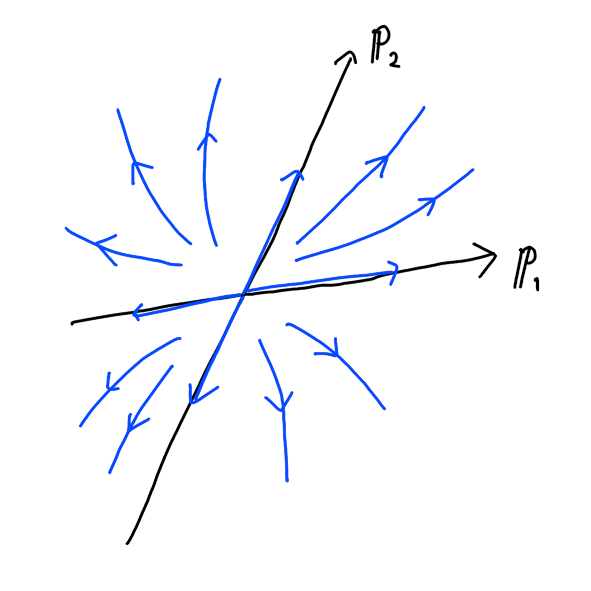
\includegraphics[height=5cm]{\assetspath assets/v1.png}
    \caption{不安定結節点}
    \label{5:fig:1}
\end{figure}

\subsection{$\lambda_1 > 0 > \lambda_2$のとき}

$e^{\lambda_1 t} \to \infty,\, e^{\lambda_2 t} \to 0\, (t \to \infty)$なので、
解のふるまいは図(\ref{5:fig:2})のようになる。
このような平衡点$P$を\textbf{鞍点}という。

\begin{figure}[H]
    \centering
    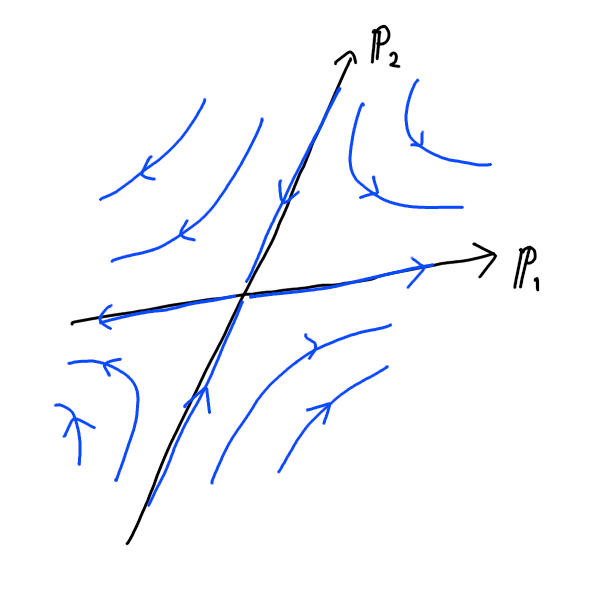
\includegraphics[width=5cm]{\assetspath assets/v2.png}
    \caption{鞍点}
    \label{5:fig:2}
\end{figure}

\subsection{$\lambda_1, \lambda_2 < 0$のとき}

$e^{\lambda_i t} \to 0\, (t \to \infty)$なので、
解のふるまいは図(\ref{5:fig:3})のようになる。
このような平衡点$P$を\textbf{安定結節点}という。

\begin{figure}[H]
    \centering
    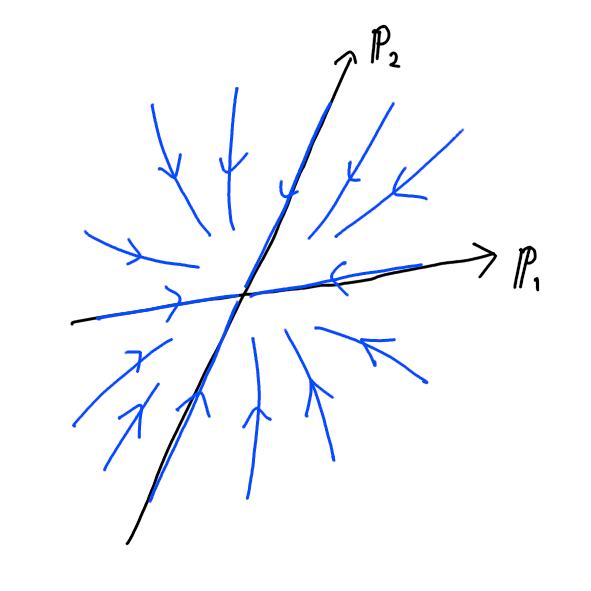
\includegraphics[width=5cm]{\assetspath assets/v3.png}
    \caption{安定結節点}
    \label{5:fig:3}
\end{figure}

\subsection{
    \texorpdfstring{%
        $\lambda_1 = \overline{\lambda_2} \not\in \R,\, \Re \lambda_i > 0$のとき%
    }{%
        %
    }%
}

解のふるまいは図(\ref{5:fig:4})のようになる。
このような平衡点$P$を\textbf{不安定渦状点}という。

\begin{figure}[H]
    \centering
    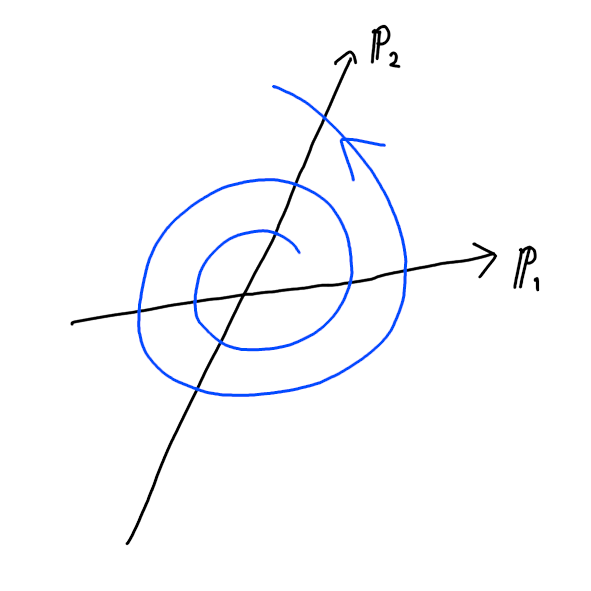
\includegraphics[width=5cm]{\assetspath assets/v4.png}
    \caption{不安定渦状点}
    \label{5:fig:4}
\end{figure}

\subsection{
    \texorpdfstring{%
        $\lambda_1 = \overline{\lambda_2} \not\in \R,\, \Re \lambda_i < 0$のとき%
    }{%
        %
    }%
}

解のふるまいは図(\ref{5:fig:5})のようになる。
このような平衡点$P$を\textbf{安定渦状点}という。

\begin{figure}[H]
    \centering
    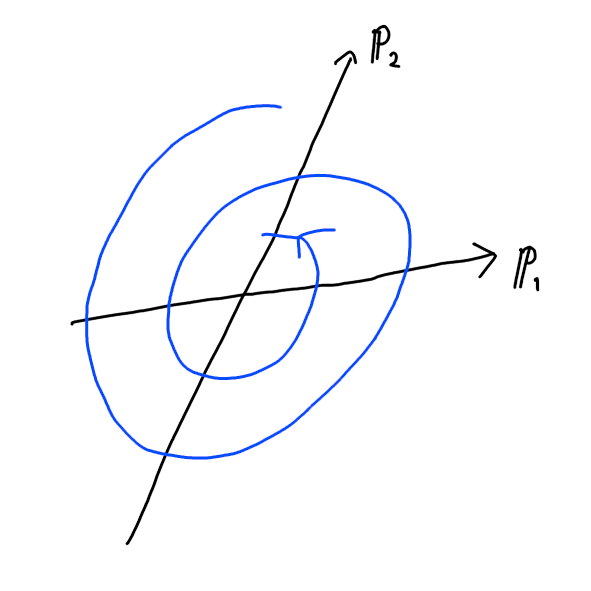
\includegraphics[width=5cm]{\assetspath assets/v5.png}
    \caption{安定渦状点}
    \label{5:fig:5}
\end{figure}

\subsection{$\Re\lambda_i = 0$の固有値があるとき}

線型化方程式の解のふるまいを用いて元の力学系の解のふるまいを判定することはできない。


\begin{problem}
    力学系
    \begin{equation}
        \begin{cases}
            x' = (1 - y) x \\
            y' = (1 + 2x) y
        \end{cases}
    \end{equation}
    の解で$x(0), y(0) > 0$をみたすものは
    $\forall t \in \R$に対し$x(0), y(0) > 0$をみたすことを示せ。
\end{problem}

\begin{problem}
    2次元力学系
    \begin{equation}
        \begin{cases}
            x' &= (1 - x - 3y) x \\
            y' &= (1 - 3x - y) y
        \end{cases}
    \end{equation}
    の平衡点の種類を判定せよ。

    解答:不安定結節点$(0, 0)$、鞍点$(1/4, 1/4)$、安定結節点$(1, 0), (0, 1)$
\end{problem}

\begin{problem}
    教科書の問5.3, 問5.4, 問5.5を読者の演習問題とする。
\end{problem}


\end{document}

\newpage
\documentclass{jlreq}
\usepackage{mymacro}
\subfiletrue
\begin{document}


\section{付録}

\subsection{感染症モデル}

授業ではSISモデルやSIRモデルなどが紹介された。
これらは$t$を陽に含まない連立1階常微分方程式、すなわち力学系である。
いずれの場合も、未知関数の総和が一定であるという条件を利用して
実質的に1本あるいは2本の連立常微分方程式に帰着させるのが基本方針である。


\ifsubfile
   \bibliographystyle{junsrt}
   \bibliography{references}
\fi
\end{document}

% ============================================================
%
% ============================================================
\newpage
\phantomsection
\addcontentsline{toc}{chapter}{演習問題の解答}
\chapter*{演習問題の解答}

\includecollection{answers}

% ============================================================
%
% ============================================================
\newpage
\phantomsection
\addcontentsline{toc}{chapter}{参考文献}
\renewcommand{\bibname}{参考文献}
\markboth{\bibname}{}
\bibliographystyle{amsalpha}
\bibliography{../mybibliography}

% ============================================================
%
% ============================================================
\newpage
\phantomsection
\addcontentsline{toc}{chapter}{記号一覧}
\printglossary[title={記号一覧}]

% ============================================================
%
% ============================================================
\newpage
\phantomsection
\addcontentsline{toc}{chapter}{索引}
\printindex

\end{document}